\documentclass[a4paper]{article}

% --- DATA ---

\def\lecture{Mathe-Zirkel Knotentheorie}
\def\authors{Linus Mußmächer}
\def\sheetNumber{00}
%\def\sumPoints{30} 

% --- PREAMBLE ---

\usepackage[german]{babel}	% language specific quotation marks etc.
% === USAGE ===

% when using this preamble, setup your environment variables like this beforehand:


% \title{Stochastik 2}  %Title of exercise 
% \def\lecture{Stochastik 2}
% \def\authors{Linus Mußmächer}
% \def\sheetNumber{02}
% \def\sumPoints{30}      % maximum number of points (leave undefined)

% then use one of these commands (german or english) to print the header:

% \makeexheaderger

% and finally use subsections for your subtasks - they will be numbered as <sheetNumber><task number> by themselves

% if you have an exercise as an external .pdf, use \includetask to include it and increase the task counter


% --- OTHER ---

\usepackage{booktabs}       % professional-quality tables
\usepackage[table]{xcolor}	% color
\usepackage{pdfpages}		% to include entire pdf pages in appendix etc.
\usepackage{enumitem}		% better custom enumerations
\setlist[enumerate, 1]{label=(\roman*)}
\usepackage{etoolbox}		% toolbox for command modification

% --- FONTS & TYPESETTING ---

\usepackage[utf8]{inputenc} % allow utf-8 input
\usepackage[T1]{fontenc}    % use 8-bit T1 fonts
\usepackage{dsfont}			% font with double lines for sets
\usepackage[german,ruled,vlined,linesnumbered,commentsnumbered,algoruled]
{algorithm2e} 				%pseudo code
\usepackage{listings}		%java code
\usepackage{csquotes}

% --- URLS ---

\usepackage[colorlinks=true, linkcolor=black, citecolor=blue, urlcolor=blue]{hyperref}   	% hyperlinks
\usepackage{url}            % simple URL typesetting

% --- MATH SYMBOLS ---

\usepackage{amsmath,amssymb}% more math symbols
\usepackage{amsfonts}       % blackboard math symbols
\usepackage{latexsym}		% more math symbols
\usepackage{chngcntr}		% more math symbols
\usepackage{mathrsfs}		% math-fonts
\usepackage{mathtools}		% more math symbols
\usepackage{nchairx}		% Waldmann package for general math symbols

% --- GRAPHICS & CAPTIONS ----

\usepackage{graphicx}		% including images
\graphicspath{ {./figs/} }
\usepackage{subcaption}		% custom caption formatting
\DeclareCaptionLabelFormat{custom}{ \textbf{#1 #2}}
\captionsetup{format=hang}
\captionsetup{width=0.9\textwidth,labelformat=custom}
\usepackage{pdfpages}		% to include entire pdf pages in appendix etc.

% --- FORMAT ---

\usepackage[a4paper]{geometry} % a4 paper
\usepackage{setspace}		% spacing
\usepackage{titlesec}
\allowdisplaybreaks			% allow page breaks within math environments

% --- CUSTOM COMMANDS ---
%Logic
\newcommand{\then}{\Rightarrow}
\newcommand{\since}{\Leftarrow}
\renewcommand{\iff}{\ensuremath{\Leftrightarrow}}

%pretty epsilon
\let\oldepsilon\epsilon
\let\epsilon\varepsilon
\let\varepsilon\oldepsilon
%pretty phi
\let\oldphi\phi
\let\phi\varphi
\let\varphi\oldphi

\newcommand{\includetask}[2][pages=-]{
    \includepdf[#1]{#2}
    \addtocounter{subsection}{1}
}

% set-up for exercise specific stuff
\ifdef{\sheetNumber}{
    \setcounter{section}{\sheetNumber}
}{}

\usepackage{titling}
\newcommand{\makeexheaderger}{
    \begin{doublespace}
        \begin{center}
            \textbf{\Large{Übungsblatt \sheetNumber}}\\
            \textbf{\Large\lecture}\\
            Abgabe von: \textbf{\authors}\\
            \today
        \end{center}
        \ifdef {\sumPoints}
        {
            \hfill  \large Punkte: $\boxed{\qquad  /\; \sumPoints}$\\
        }{}
    \end{doublespace}
}

\newcommand{\makeexheadereng}{
    \begin{doublespace}
        \begin{center}
            \textbf{\Large{Exercise Sheet \sheetNumber}}\\
            \textbf{\Large\lecture}\\
            Abgabe von: \textbf{\authors}\\
            \today
        \end{center}
        \ifdef {\sumPoints}
        {
            \hfill  \large Points: $\boxed{\qquad  /\; \sumPoints}$\\
        }{}
    \end{doublespace}
}
\usepackage[fontsize=12pt]{fontsize}
\usepackage{parskip}
\usepackage{calc}

\newboolean{wordblank}
\setboolean{wordblank}{true}
\newcommand{\blankword}[1]{\ifthenelse{\boolean{wordblank}}{\underline{\phantom{#1#1}}}{#1}}



\geometry{top=2.0cm, bottom=2.0cm, left=2.0cm, right=2.0cm}

\begin{document}
    \pagestyle{empty}

    \begin{tabular*}{\textwidth}{L{0.65\textwidth} R{0.35\textwidth}}
        \multirow{4}{*}{
\includegraphics[height=2.1cm]{img/unimarke_Vektor_CMYK.eps} \qquad 
\includegraphics[height=2.1cm]{img/LOGO-wuemax-color-2022.png}} & \textsc{Universität Würzburg}  \\
        & \textsc{Institut für Mathematik}  \\
        & \textsc{wümax}  \\
        & \textsc{Linus Mußmächer}
    \end{tabular*}

    \begin{doublespace}
        \begin{center}
            \textsc{\large{Mathe-Zirkel}}\\
            17. Juni 2023 \\
            \textbf{\Large{Knotentheorie}}
        \end{center}
    \end{doublespace}


    Ein \textbf{Knoten} ist ein Weg im Raum, der sich im Raum \blankword{niemals} selbst schneidet.

    Ein Knoten in der Mathematik unterscheidet sich von einem normalen Knoten dadurch, dass \\
    \blankword{seine Enden miteinander verbunden sind}.

    Zwei Knoten sind gleich (äquivalent), wenn man sie durch \blankword{stetige} Bewegungen gleich machen kann. Dabei darf man den Knoten\\
    \blankword{bewegen, drehen, biegen, zerren, stauchen},\\
    aber niemals\\
    \blankword{zerschneiden, durch sich selbst schieben}.

    \textit{Einige Knoten}:
    \begin{center}
    \begin{tabular}{c c c c}
        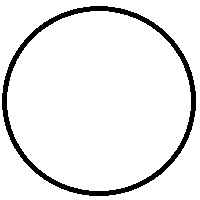
\includegraphics[width=3.5cm]{img/knots0.png} &
        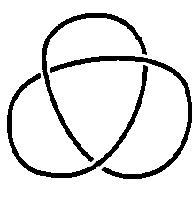
\includegraphics[width=3.5cm]{img/knots1.png} &
        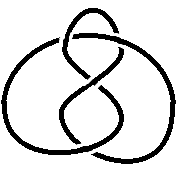
\includegraphics[width=3.5cm]{img/knots2.png} &
        \fbox{\phantom{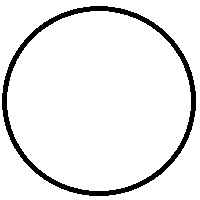
\includegraphics[width=3.5cm]{img/knots0.png}}} \\
        \blankword{Unknoten} &
        \blankword{Kleeblatt} &
        \blankword{Achter} &
        \blankword{Eigener}
    \end{tabular}
    \end{center}

    Malen wir einen Knoten wie oben auf ein Blatt Papier, so nennt man diese Zeichnung eine \blankword{Projektion} des Knotens.

    Es gibt immer mehrere Möglichkeiten, einen Knoten zu zeichnen.

    \textit{Einige Zeichnungen des Achterknotens}:
    \begin{center}
        \begin{tabular}{c c c}
            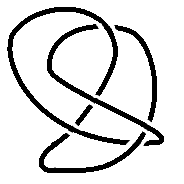
\includegraphics[width=3.5cm]{img/eight0.png} &
            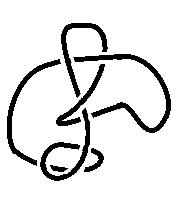
\includegraphics[width=3.5cm]{img/eight1.png} &
            \fbox{\phantom{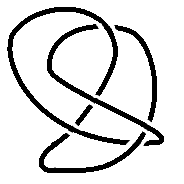
\includegraphics[width=3.5cm]{img/eight0.png}}}
    \end{tabular}
    \end{center}

    % \begin{tabular*}{\textwidth}{L{0.99\textwidth - 3cm} R{3cm}}
    % Mehrere Knoten, die miteinander verbunden sind, nennt man eine \rule{3 cm}{0.5pt}. Links sieht man die \textit{Borromäischen Ringe}. & 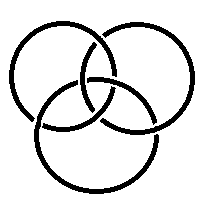
\includegraphics[width=2.5cm]{img/ring.png}
    % \end{tabular*}

\end{document}